\chapter{Cryptographic Protocols and Key Distribution}

\section{Communication Protocols}

It is a system that allows two or more entities to exchange information. It defines the rules, syntax, semantics and synchronization of communication and possible error recovery methods. It can be implemented by hardware, software, or a combination of both. It uses messages with well-defined formats (syntax) and each message has an exact meaning intended to elicit a response from a range of possible responses pre-determined for that particular situation (semantics). The specified behaviour is typically independent of how it is to be implemented.

\section{Cryptographic Protocol}

It is a communication protocol (usually a small one, meaning that its specification is typically quite compact, e.g., few exchange of messages in given formats) designed to secure communication (various security goals) by using cryptographic primitives (e.g., ciphers, hash functions, ...).

Typical security goals/properties
\begin{itemize}
	\item Secrecy: May an intruder learn some secret message between the two honest participants Alice and Bob?
	\item Authentication: Is the agent Alice really talking to Bob?
	\item Non-repudiation: Alice sends a message to Bob. Alice cannot later deny having sent this 	message. Similarly, Bob cannot deny having received the message.
\end{itemize}


What do we mean by "The specified behavior [of a protocol] is typically independent of how it is to be implemented"? Observe that you really want to specify a protocol independently of its implementation because you want to abstract away a lot of details that are present in an implementation: type of processors used by the entities involved in the protocol, operating systems, programming language, libraries. We focus only on the essence of the cryptographic protocol, understand if it satisfies the security goal, and then consider the problem of implementing it.
The problem admits at least two possible solutions that have in common one feature, namely that the syntax and semantics of (cryptographic) protocols together with their security goals can be precisely described by using appropriate mathematical objects.
In this way, it is possible to prove (in a mathematical way) that a certain protocol achieves a security goal under the assumption that a characterization of the attacker capabilities is also included in the specification of the protocol. Typically, the attacker capabilities that are considered in the context of cryptographic protocols are the following: an (active) attacker can: 
\begin{itemize}
	\item intercept all messages sent on the network
	\item compute messages
	\item send messages on the network
\end{itemize}

So we say that the attacker is the network, or that the attacker carries the message.
Session: is set of message exchange between entities that relates logically to the same protocol specification. We'll see that a protocol can be instantiated to a specific session.
We characterize the attacker based off of how can he interfere with the properties of the cryptographic protocol. We take into consideration the Dolev-Yao (or Formal) adversary model. Unlike in the real world, the adversary can neither manipulate the encryption's bit representation nor guess the key. The attacker may, however, re-use any messages that have been sent and therefore become known. The attacker can encrypt or decrypt these with any keys he knows, to forge subsequent messages. 

In this model we assume that the cryptographic primitives are black-boxes and that the messages are expressions built out of the cryptographic primitive. Additionally we say that cryptographic primitive cannot be broken or, equivalently, we assume that cryptography is perfect.

Needless to say this is an abstraction and maybe a coarse abstraction that ignores all the weaknesses that may be existing in available cryptographic primitives. This implies that a proof of the security of a certain protocol in this model holds under the assumption that the attacker does not attempt to break the cryptographic primitives and, of course, that the protocol implementation correctly implements its specification.


There are other models, such as the computation model that assumes the following:
\begin{itemize}
	\item The messages are bit-strings
	\item The cryptographic primitives are functions on bit-strings
	\item The attacker is any probabilistic (polynomial-time) Turing machine
\end{itemize}

A probabilistic Turing machine is a non-deterministic Turing machine that chooses between the available transitions at each point according to some probability distribution (roughly by tossing a coin at each step in the computation).

The main difference with the Dolev-Yao model is that cryptographic primitives are no more perfect but are functions operating on bit-strings which is a less coarse abstraction; however, notice that it is still an abstraction since bit-strings are mathematical objects that are quite different from the bit-strings datatypes that we may find in programming languages. A probabilistic (polynomial-time) Turing machine characterizes the capabilities of a computationally constrained attacker that can solve problems using randomized polynomial time algorithms including those required to break a certain cryptographic primitive.
Despite being more realistic than the Dolev-Yao model, the computational model still ignores several details that should be considered when implementing a cryptographic protocol including side channel attacks such as: timing, power consumption, noise, physical attacks against smart card.
A side-channel attack aims to gather information from or influence the execution of a system by measuring or exploiting indirect effects of the system or its hardware rather than targeting the program or its code directly. In other words, side channel attacks do not exploit weaknesses in the implemented system but rather gain information from the execution of the system itself.

An attack in the Dolev-Yao model implies a (practical) attack in the computational model. A proof in the Dolev-Yao model does not always imply a proof in the computational model.
The Dolev-Yao model allows for automated verification. Most proofs in the computational model are manual.



\section{Security issues in protocols because of symmetric ciphers}

Assume that a large number of people, processes, or systems that want to communicate with one another in a secure fashion and that this group of people/processes/systems is not static, i.e. individual entities may join or leave the group at any time. The naive solution would be to have point-to-point key establishment, so each party physically exchange an encryption key with every one of the other parties, but these way we need a quadratic $N*(N-1) / 2$ number of keys. But each entity has many keys to manage and has to manage them in an appropriate way. This is not feasible for large groups, especially if the group membership evolves over time and keys have to be rotated frequently.

Secondly we need a way of exchanging the first key that then can be used by the two parties to communicate securely. So we need to introduce the notion of session/ephimeral key. Point-to-point key establishment has a few pros and cons: in terms of security if subject is compromised only its communications are compromised; communications between two other subjects are not compromised, on the other side it has poor scalability as the number of keys is quadratic in the number of subjects and has poor handling of dynamic topologies: a new member joining and a member leaving affect all current members. For large networks this becomes impractical and we need to design an alternative solution based on a trusted 3rd party that mediates the establishment of a secure connection.

\section{Key Distribution Center}

Key distribution as a trusted 3rd party. Each entity needs to change a master key with the key distribution center, so we need only a linear number of keys. Provide every group member with a single key, called the master key, for securely communicating with a key distribution center (KDC). When $A$(lice) wants to establish a secure communication link with $B$(ob), $A$(lice) requests a session key from KDC for communicating with $B$(ob). But there are a few issues we need to solve:
\begin{itemize}
	\item Assuming that $A$ is the initiator of a session-key request to KDC, when $A$ receives a response from KDC, how can $A$ be sure that the sending party for the response is indeed the KDC?
	\item Assuming that $A$ is the initiator of a communication with $B$, how does $B$ know that some other party is not masquerading as $A$?
	\item How does $A$ know that the response received from $B$ is indeed from $B$ and not from someone else masquerading as $B$?
	\item What should be the lifetime of the session key acquired by $A$ for communicating with B?
\end{itemize}

\subsection{Needham-Schroeder key distribuition}

A party $A$ wants to establish a secure communication link with another party $B$ \ref{fig:needhamschroederprotocol}. Both $A$ and $B$ possess master keys $K_{AS}$ and $K_{BS}$, respectively, for communicating privately with a key distribution center (KDC). Needham-Schroeder is a shared-key authentication protocol designed to generate and propagate a session key, i.e., a shared key for subsequent symmetrically encrypted communication. Notice that there is no public key infrastructure in place and we've made the assumption that both $A$ and $B$ have a shared communication key with S. It is crucial that the key shared between $A$ and $S$ ($K_{AS}$) is protected otherwise anyone can impersonate $A$ (similarly for $B$).
$S$ is the server that is the trusted 3rd party in this communication and it allows pair of users to establish a session key. Each user shares a long-term key, a priori with $S$. The overall number of long-term keys is linear in the number of users. S maintains a database containing pairs associating an identifier of a user and the key shared between the user and S. It has to be considered as an honest participant of the key distribution protocol. This creates a single point of failuere so we need a way of protecting keys stored in the KDC. Usually an hierarchical structure of KDCs is preferred, because it limits the damage of a faulty KDC. 

Needham-Schroeder uses nonces (numbers used once), that are randomly generated values included in messages. If a nonce is generated and sent by $A$ in one step and returned by B in a later step, $A$ knows that $B$ message is fresh and not a replay from an earlier exchange, the only assumption is that it has not been used in any earlier interchange. The nonce generated by $A$ will be noted as $N_{A}$ and the one from $B$ will ne noted as $N_{B}$. The nonce can be seen as a session identifier, i.e. an identifier of the particular exchange of messages that A and B are going to have using a suitably shared session key, unique to that session. $K_{AB}$ is a symmetric, generated key, which will be the session key of the session between $A$ and $B$.

\begin{figure}
	\centering
	\includegraphics[width=0.7\linewidth]{Images/Chapter4/Needham–Schroeder_protocol}
	\caption{Needham–Schroeder Protocol}
	\label{fig:needhamschroederprotocol}
\end{figure}

The procedure has these steps:
\begin{enumerate}
	\item $A$ contacts $S$, by sending its identifier $A$, the identifier of $B$ and then a nonce $N_{A}$.
	\item $S$ responds by sending $N_{A}$, $B$, and creates $K_{AB}$. Then adds $K_{AB}$ and $A$ encrypted with $K_{BS}$ and encrypts the whole message with $K_{AS}$.
	\item $A$ then sends $K_{AB}$ and $A$ encrypted with $K_{BS}$ to $B$. At this point $B$ knows that $A$ wants to communicate with them, and also knows the session key $K_{AB}$. Then $B$ sends $N_{B}$ encrypted with $K_{AB}$ to $A$.
	\item $A$ sends $N_{B} - 1$ encrypted with the session key $K_{AB}$ to $B$.
\end{enumerate}

This protocol is vulnerable to an attack called Replay attack where if the attacker compromises $K_{AB}$ it can then send the message $K_{AB}$ and $A$ encrypted with $K_{BS}$ to $B$, who who will accept it, being unable to tell that the key is not fresh, because it doesn't contain nonces. At this point $B$ believes that $A$ sent that message all will send back $N_{B}$ encrypted with $K_{AB}$ to the attacker that will answer accordingly. Now the attacker has successfully impersonated $A$.

This flaw is fixed in the Kerberos protocol by the inclusion of a timestamp.
\begin{enumerate}
	\item $A$ contacts $S$, by sending its identifier $A$, the identifier of $B$.
	\item $S$ responds by sending $T$, $B$, and creates $K_{AB}$. Then adds $K_{AB}$, $A$, and $T$ encrypted with $K_{BS}$ and encrypts the whole message with $K_{AS}$.
	\item Then $A$ sends $K_{AB}$, $A$, and $T$ encrypted with $K_{BS}$ to $B$.
\end{enumerate}

But the clock on each machine can drift, and introduces the problem again. There needs to be an infrastructure to synchronize clocks! This does not scale easily, but it is fine with few devices.

\section{Kerberos}
Kerberos operates on the principle of shared secret keys. Its goal is to establish a direct authenticated and confidential communication link between the host (where a print request originates) and the printer. Since printers generally are rudimentary when it comes to general purpose computing, you may not expect a printer to contain all of the software that generally is required (such as the SSL/TLS libraries) for establishing such links.

In Kerberos there is a service which sole purpose is to authenticate. Both users and services implicitly trust the Kerberos Authentication Service ($AS$) that mediates their interaction. For this to work, both the user and the service must have a shared secret key registered with the $AS$. Such keys are called long-term keys, since they last for weeks or months.

There are three basic steps involved in authenticating a user to an end service
\begin{itemize}
	\item The user $U$ sends a request to the $AS$, asking it to authenticate $U$ to the service $S$. This request consists only of the service's name, although in practice, it contains some other information (recall the nonce in the Needham-Schroeder protocol).
	\item The $AS$ prepares to introduce the user $U$ and the service $S$ to each other, it generates a new, random secret key that will be shared only by $U$ and $S$ and it sends the user a two-part message, one part contains the random key along with the service's name, encrypted with the user's long-term key, the other part contains that same random key along with the user's name, encrypted with the service long-term key. Notice that at this point, only the user $U$ knows the session key, provided it really is the user $U$ and knows the appropriate long-term key.
	\item User $U$ generates a fresh message (called authenticator) and encrypts it with the session key, then sends the authenticator, along with the ticket, to the service. The service $S$ decrypts the ticket with its long-term key to recover the session key. In turn, the session key is used to decrypt the authenticator. The service $S$ trusts the $AS$, so it knows that only the legitimate user could have created such an authenticator and this completes the authentication of the user to the service. If the user $U$ want the service $S$ to be authenticated in return, then the service $S$ takes $N_{ab}$ from the authenticator, adds the service's own name to it, and encrypts the whole message with the session key. This is then returned to the user $U$.
\end{itemize}

The main difference between the Needham-Schroeder protocol and the Kerberos protocol is that the latter makes a distinction between the clients, on the one hand, and the service providers, on the other.

One of the inconveniences of using a password is that each time you access a service, you have to type it in. Kerberos resolves the last problem by introducing a new service, called the ticket granting server ($TGS$). The purpose of the TGS is to add an extra layer of indirection so that the user only needs to enter a password once and the ticket and session key obtained from that password are used for all further tickets \ref{fig:kerberos}. The client can not communicate directly with the $TGT$, it has to ask the $KDC$ for a Ticket Granting Ticket ($TGT$). Afer having this ticket it can request any service ticket, and communicate with that service with that ticket \ref{fig:kerberos1} \ref{fig:kerberos-keys} \ref{fig:kerberos2}.


\begin{figure}
	\centering
	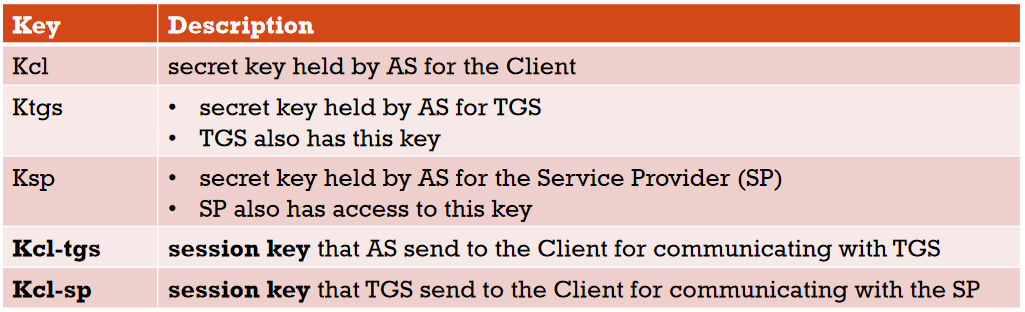
\includegraphics[width=0.7\linewidth]{Images/Chapter4/kerberos-keys}
	\caption{}
	\label{fig:kerberos-keys}
\end{figure}

\begin{figure}
	\centering
	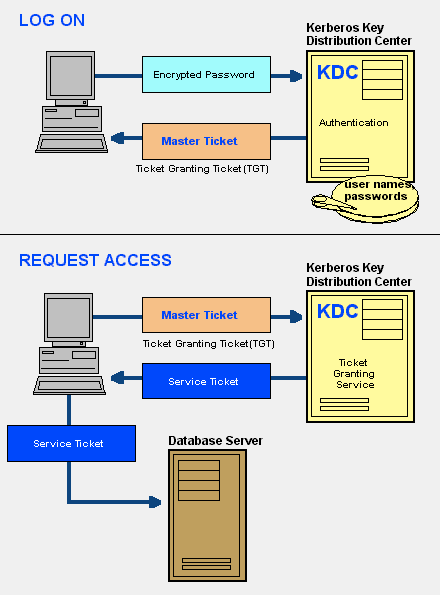
\includegraphics[width=0.7\linewidth]{Images/Chapter4/kerberos}
	\caption{}
	\label{fig:kerberos}
\end{figure}

\begin{figure}
	\centering
	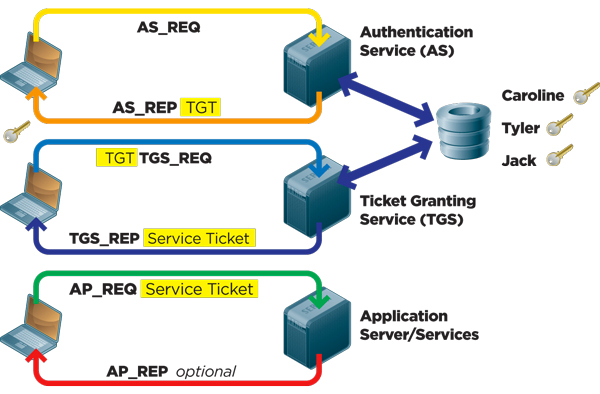
\includegraphics[width=0.7\linewidth]{Images/Chapter4/kerberos1}
	\caption{}
	\label{fig:kerberos1}
\end{figure}

\begin{figure}
	\centering
	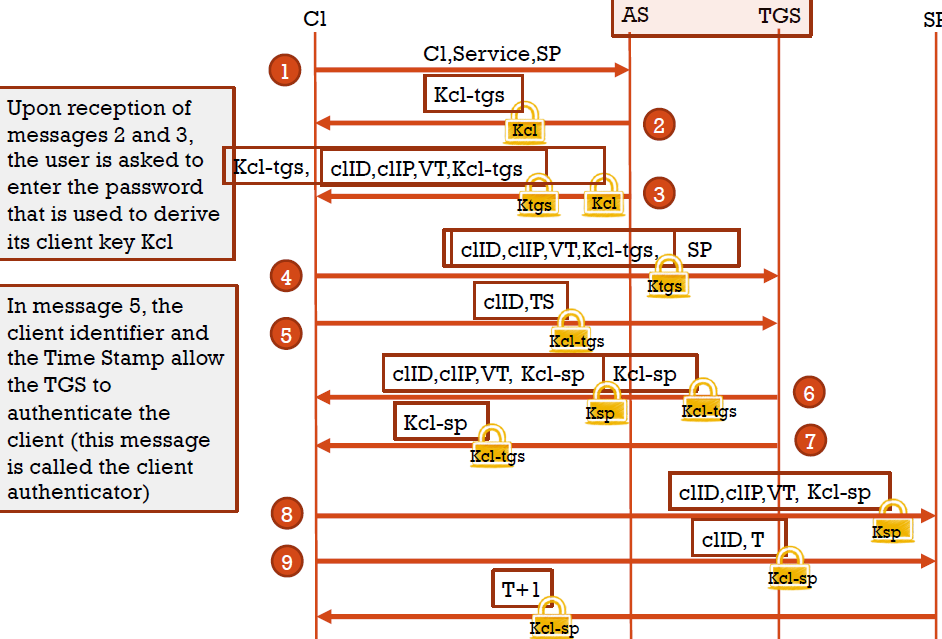
\includegraphics[width=0.7\linewidth]{Images/Chapter4/kerberos2}
	\caption{The protocol}
	\label{fig:kerberos2}
\end{figure}

\begin{enumerate}
	\item Client sends a request in plain text to the $AS$, this request is for a service that the Client expects from the $SP$
	\item AS sends back to the Client the following two messages encrypted with $K_{cl}$. In the database maintained by $AS$, $K_{cl}$ is specific to the Client and will remain unchanged as long as the client does not alter its password. This encryption key is not directly known to the Client. The two messages are: a session key $K_{cl-tgs}$ that the client can use to communicate with $TGS$ and a Ticket-Granting Ticket ($TGT$) that is meant for delivery to $TGS$ including the client user ID ($clID$), client network address ($clIP$) a validation time ($VT$) and the same $K_{cl-tgs}$ session key. The ticket is encrypted with the $K_{TGS}$ secret key that the $AS$ server maintains for $TGS$
	\item After step 3 and before step 4 the client is asked to provide the password in a dialog box. Then the password is converted into the $K_{cl}$ if it is correct. This key is then used to extract the session key $K_{cl-tgs}$ and the ticket meant for $TGS$ from the information received from $AS$.
	\item In steps 4 and 5 the client sends the following two messages to $TGS$: the encrypted ticket meant for $TGS$ followed by the ID of the requested service and a Client Authenticator that is composed of the client ID and the timestamp, both encrypted with the $K_{cl-tgs}$ session key.
	\item Before steps 6 and 7 $TGS$ recovers the ticket from message 4 above, from the ticket, it recovers the $K_{cl-tgs}$ session key. The $TGS$ then uses the session key to decrypt message 5 above that allows it to authenticate the Client
	\item in steps 6 and 7 $TGS$ sends back to the Client the following two messages: a Client-to-Service Provider ticket that consists of the Client ID ($clID$), the Client network address ($clIP$), the validation time ($VT$), a session key $K_{cl-sp}$ for the Client and the Service Provider encrypted with the $K_{sp}$ key that is known to $TGS$ and another message containing the same $K_{cl-sp}$ session key encrypted with the $K_{cl-tgs}$ session key
	\item Before steps 8 and 9 the client recovers the ticket meant for the service provider with the $K_{cl-tgs}$ session key
	\item In steps 8 and 9 the client next sends the following two messages to the service provider: the Client-to-ServiceProvider ticket that was encrypted by $TGS$ with the $K_{sp}$ key and an authenticator that consists of the Client ID and the timestamp, encrypted with the $K_{cl-sp}$ session key
	\item Before step 10 the $SP$ decrypts the ticket with its own $K_{sp}$ key, it extracts the $K_{cl-sp}$ session key from the ticket and then uses the session key to decrypt message 9 received from the client.
	\item In step 10 $SP$ sends to the Client a message that consists of the timestamp in the authenticator received from the Client plus one, encrypted with $K_{cl-sp}$
	\item After step 10 the client decrypts the message received from the Service Provider using the $K_{cl-sp}$ session key and makes sure that the message contains the correct value for the timestamp. If that is the case, the client can start interacting with the Service Provider
\end{enumerate}

\section{Kerberos Security Issues}
The primary way in which an attacker will attempt to compromise a Kerberos Infrastructure would be to attack the Kerberos servers. If an attacker can gain root access to a KDC, the attacker will have access to the database of shared keys of the principals. 

Since the security of Kerberos authentication is in part based upon the time stamps of tickets, it is critical to have accurately set clocks on Kerberos servers. It is advisable to set a short lifetime for tickets to prevent attackers from performing successful brute force attacks or replay attacks. If one allows for server clocks to drift, the network will become vulnerable to such attacks. If clocks are not synchronized within a reasonable time window, Kerberos will report fatal errors and refuse to function.  machine with an inaccurate clock will be failed by the KDC in authentication attempts due to the time difference with the KDC's clock.
The Network Time Protocol (NTP) is available for the time synchronization of servers.



\section{Protocol Specification \& Analysis}
We want to give structured methods to prove or disprove that a given protocol satisfies a certain security property and achieves a certain security goal despite an attacker.

It is already difficult to understand the security of certain protocols, of the absence of a problem. Even with few messages, can we argue no attack is possible? We want evidence that the protocol does exactly what we designed, and we have achieved the security goal.

\subsection{Digression on notation}

Alice\&Bob–notation is commonly used to describe security protocols as sequences of message exchange steps of the form: $\mathcal{A} \rightarrow \mathcal{B}: \mathcal{M}$  where $\mathcal{A}$ and $\mathcal{B}$ are the parties involved in the message exchange and $\mathcal{M}$ is the message being exchanged.
But there are some issues that need clarification:
\begin{itemize}
	\item [1.] Need to make explicit what is known (public, private) before a protocol run, and what is to be generated freshly during a protocol run (e.g. nonces).
	\item [2.] Need to make explicit which checks the individual principals are expected to carry out on the reception of messages. This is because the message sent by $\mathcal{A}$ may never be received by $\mathcal{B}$, or $\mathcal{B}$ might receive a different message from the one sent by $\mathcal{A}$.
	\item [3.] Principals act concurrently, in contrast to the apparently sequential idealized execution of a run according to a narration. So messages could be received in different order from the expected one.
	\item [4.] Concurrency occurs also at the level of different protocol sessions, which may happen to be executed simultaneously while sharing principals across.
\end{itemize}

A more precise characterization of $\mathcal{A} \rightarrow \mathcal{B}: \mathcal{M}$ is that $\mathcal{A}$ asynchronously sends $\mathcal{M}$ towards $\mathcal{B}$, that is then received by $\mathcal{B}$. Finally $\mathcal{B}$ checks that the message received is the intended one by checking the properties of the message (e.g. the gained knowledge is consistent with previously acquired knowledge).

Due to the distributed nature of the system, protocols are highly asynchronous. A party to a protocol does not know anything about the current run of the protocol except the messages it has received and sent. Except for the initiator, other parties will not even know that they are participating until they receive their first message.

There are many different attacks that can be performed on an exchange of messages, and these attacks boil down to these questions:
\begin{itemize}
	\item Are both authentication and secrecy assured?
	\item Is it possible to impersonate one or more of the parties?
	\item Is it possible to interject messages from an earlier exchange (replay attack)?
	\item What tools can an attacker deploy with which capabilities?
	\item If any key is compromised, what are the consequences?
\end{itemize}

During protocol design we consider the Dolev-Yao model, in which the attacker can overhear, intercept, and synthesize any message and is only limited by the constraints of the cryptographic methods used. In other words: "the attacker carries the message” but it cannot break the cryptographic primitives that are considered perfect. The protocol should be robust in the face of such a determined and resourceful attacker.

\section{Verification of cryptographic protocols}

Protocols can be notoriously difficult to get correct. Protocols often depend on assumptions that are not clearly stated. It would be nice to be able to reason with mathematical rigour about protocol correctness.

There are three approaches to protocol verification:
\begin{itemize}
	\item Belief logic allow reasoning about what principals within the protocol should be able to infer from the messages they see. Allows abstract proofs, but may miss some important flaws
	\item State exploration methods (model checking) treat a protocol as a state machine and conduct an exhaustive search checking that all reachable states are safe. Is automated \href{https://tamarin-prover.github.io/manual/book/001_introduction.html}{Tamarin}.
	\item Theorem proving uses induction over potential traces of protocol execution
\end{itemize}

\subsection{Belief Logic}

A belief logic is a formal system for reasoning about beliefs. Any logic consists of a set of logical operators and rules of inferences that allows us to symbolically derive true statements.

Write mathematical expression, that describes the state of various entities (example: entity knows a key shared with another entity). A mathematically precise language two write expressions to represent states. It is made of inference rules, that allows to derive (infer) other expressions. 

\subsection{Ban Logic}

Introduced in 1989, after its inventors: Burrows, Abadi, Needham. It is based on an agreed set of deduction rules for formally reasoning about the authentication protocols and is often referred to as a logic of authentication. It is a mathematically rigorous method for verifying that two principals (people, computer, services) are entitled to believe they are communicating with each other and not the intruders. The logic cannot prove that a protocol is wrong, i.e. to disprove that a security goal cannot be achieved. However, if one can not prove a protocol correct, then it is wise to consider that protocol with great suspicion.
It helps clarify the protocol’s assumptions by formally stating them. This is a general phenomenon that is intrinsic to the formalization process, i.e. the fact of using strictly specified inference rules immediately points out which hypotheses are missing.

One assumption that we make in the Needham-Schroeder is that $N_A$ and $N_B$ is a nonce ($N_A$ is a nonce to $A$, because $A$ uses an algorithm to generate every time fresh nonces, but how can $B$ and $S$ know if $A$ generated it in a correct way, so they have to trust $A$), also that $K_{AB}$ is fresh, never seen before.

It is a logical systems based on principal beliefs and their evolution after message exchanges: it concentrates on the beliefs of trustworthy parties involved in the protocol and the evolution of these beliefs through communication processes. A logical system is a deductive system together with additional axioms and a semantics. A deductive system consists of the axioms and rules of inference that can be used to derive theorems of the system. An axiom is a statement that is taken to be true, to serve as a premise or starting point for further reasoning and arguments.
Example: It is possible to draw a straight line from any point to any other point. An inference rule is a function which takes premises, analyzes their syntax, and returns a conclusion for example Modus Ponens.
The semantics gives the meaning to the expressions of the deductive system.

\begin{figure}
	\centering
	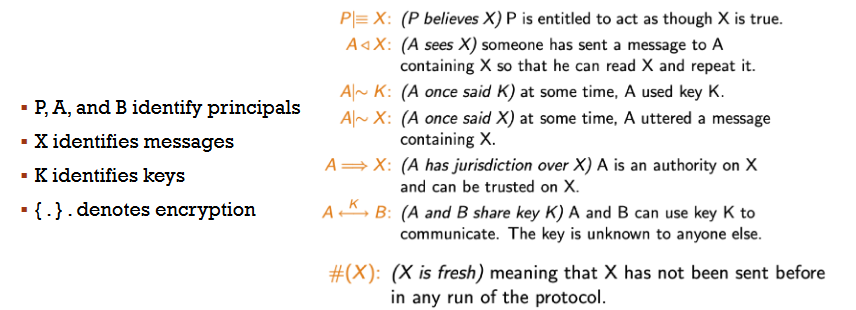
\includegraphics[width=0.7\linewidth]{Images/Chapter4/ban_logic}
	\caption{Ban logic operands}
	\label{fig:banlogic}
\end{figure}

Principals are entities participating in the message exchange.

\subsection{Ban logic rules}

\subsubsection{Rule 1}
\begin{figure}
	\centering
	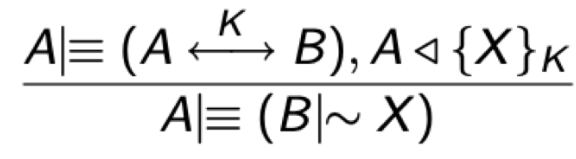
\includegraphics[width=0.3\linewidth]{Images/Chapter4/ban_logic_rule1}
	\caption{Rule 1}
	\label{fig:banlogicrule1}
\end{figure}

A believes that A and B share the key K, A sees the message with a format X encrypted with key K. So A believes that B created that message. So A belives that that message comes from B, because no one else knows the shared key K other than B, because we are using symmetric cryptography \ref{fig:banlogicrule1}.

\subsubsection{Rule 2}

\begin{figure}
	\centering
	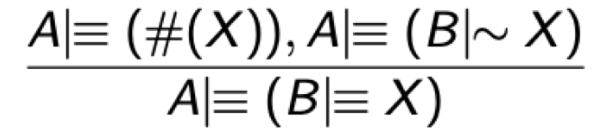
\includegraphics[width=0.3\linewidth]{Images/Chapter4/ban_logic_rule2}
	\caption{Rule 2}
	\label{fig:banlogicrule2}
\end{figure}

A believes that X is fresh (X is the nonce), A believes that B sent a message containing X. A believes everything said by B because it was said by B with the fresh nonce \ref{fig:banlogicrule2}.

\subsubsection{Rule 3}

\begin{figure}
	\centering
	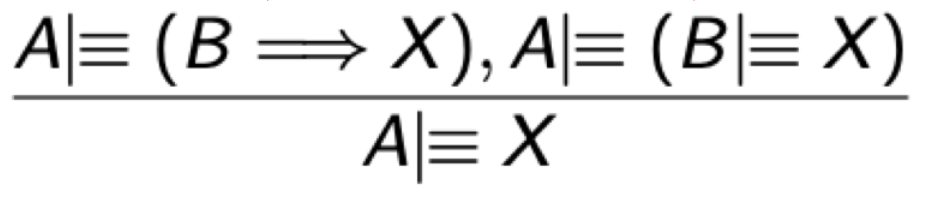
\includegraphics[width=0.3\linewidth]{Images/Chapter4/ban_logic_rule3}
	\caption{Rule 3}
	\label{fig:banlogicrule3}
\end{figure}

A believes B is trusted in saying message X, A believes that B believes X, A believes X \ref{fig:banlogicrule3}.

\subsection{Protocol analysis}
The steps of BAN logic to analyse the original protocol are as follows:
\begin{enumerate}
	\item The protocol is transformed into some idealized form
	\item Identify initial assumptions in the language of BAN logic
	\item Use the axioms and rules of the logic to deduce new expressions
	\item Interpret the statements proved by the process: are the goals achieved?
\end{enumerate}

Authentication rests on communication protected by shared session key, so the goals of authentication may be reached between A and B if there is a shared K such that:
\begin{itemize}
	\item Key authentication: $ A \mid \equiv A \Leftrightarrow^K B $ and $ B \mid \equiv A \Leftrightarrow^K B $
	\item Key confirmation: $ A \mid \equiv B \mid \equiv A \Leftrightarrow^K B $ and $ B \mid \equiv A \mid \equiv A \Leftrightarrow^K B $
	\item Key freshness: $ A \mid \equiv \# (A \Leftrightarrow^K B)$ and $ B \mid \equiv \#(A \Leftrightarrow^K B)$
\end{itemize}

\section{Application to Needham-Schroeder}
\subsection{Formalization}

Steps to formalization: \ref{fig:formalization1}, \ref{fig:formalization21}, \ref{fig:formalization22}, \ref{fig:formalization23}.
\begin{figure}
	\centering
	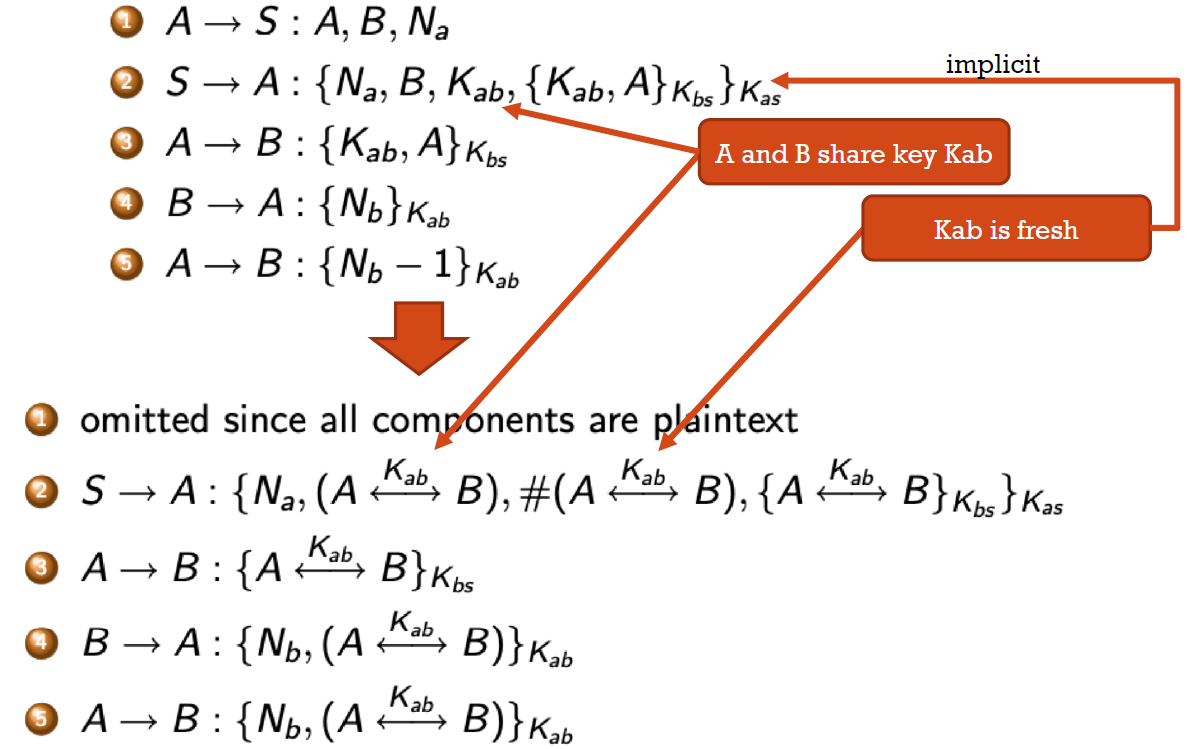
\includegraphics[width=0.7\linewidth]{Images/Chapter4/formalization1}
	\caption{Formalization 1}
	\label{fig:formalization1}
\end{figure}




Regarding \ref{fig:formalization21}:
\begin{itemize}
	\item $K_{AS}$ is a shared key by $A$ and $S$; both $A$ and $S$ believes this
	\item $K_{BS}$ is a shared key by $B$ and $S$; both $B$ and $S$ believes this
	\item $K_{AB}$ is a shared key by $A$ and $B$; only $S$ believes this
\end{itemize}

\begin{figure}
	\centering
	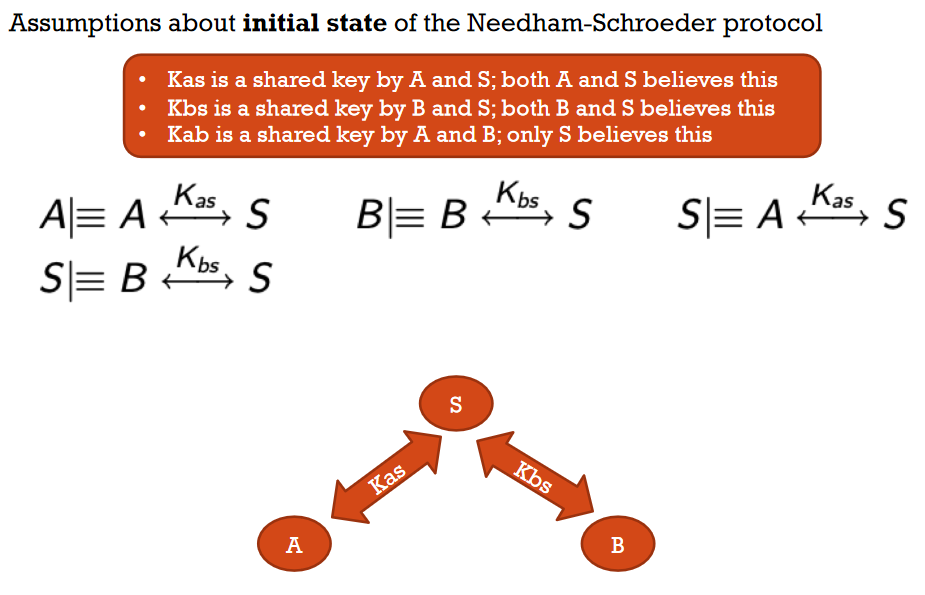
\includegraphics[width=0.7\linewidth]{Images/Chapter4/formalization21}
	\caption{Formalization 2.1}
	\label{fig:formalization21}
\end{figure}

Regarding \ref{fig:formalization22}:
for any key $K$: $S$ is an authority to say that $K$ is a shared key by $A$ and $B$, and it is trusted to say this; both $A$ and $B$ believes this. $S$ is an authority to say that $K$ is a fresh shared key by $A$ and $B$, and it is trusted to say this; only $A$ believes this.

\begin{figure}
	\centering
	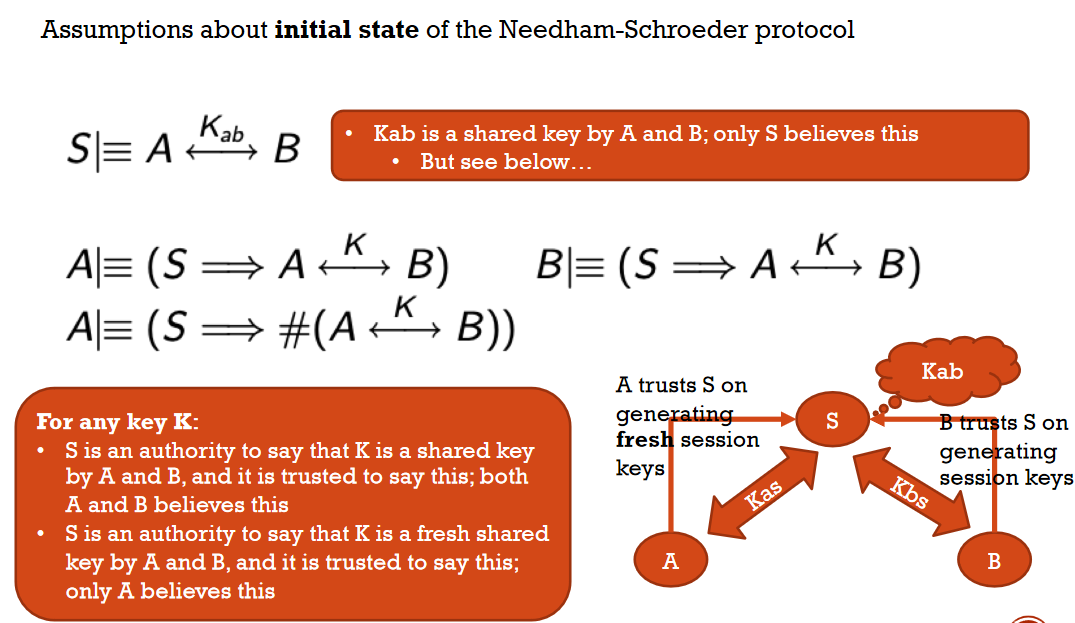
\includegraphics[width=0.7\linewidth]{Images/Chapter4/formalization22}
	\caption{Formalization 2.2}
	\label{fig:formalization22}
\end{figure}


Regarding \ref{fig:formalization23}:
\begin{itemize}
	\item $N_{A}$ is fresh and $A$ believes this
	\item $N_{B}$ is fresh and $B$ believes this
	\item $K_{AB}$ is a fresh shared key by $A$ and $B$; $S$ believes this. 
\end{itemize}


Regarding \ref{fig:formalization23}: For any key $K$, $B$ believes that $K$ is a fresh shared key by $A$ and $B$. 
Notice that $A$ and $B$ trusts $S$ in different ways: $A$ trusts also the fact that $S$ is able to generate fresh keys, $B$ does not trust this and assumes that any shared key with $A$ is fresh. This paves the way to the attack.

\begin{figure}
	\centering
	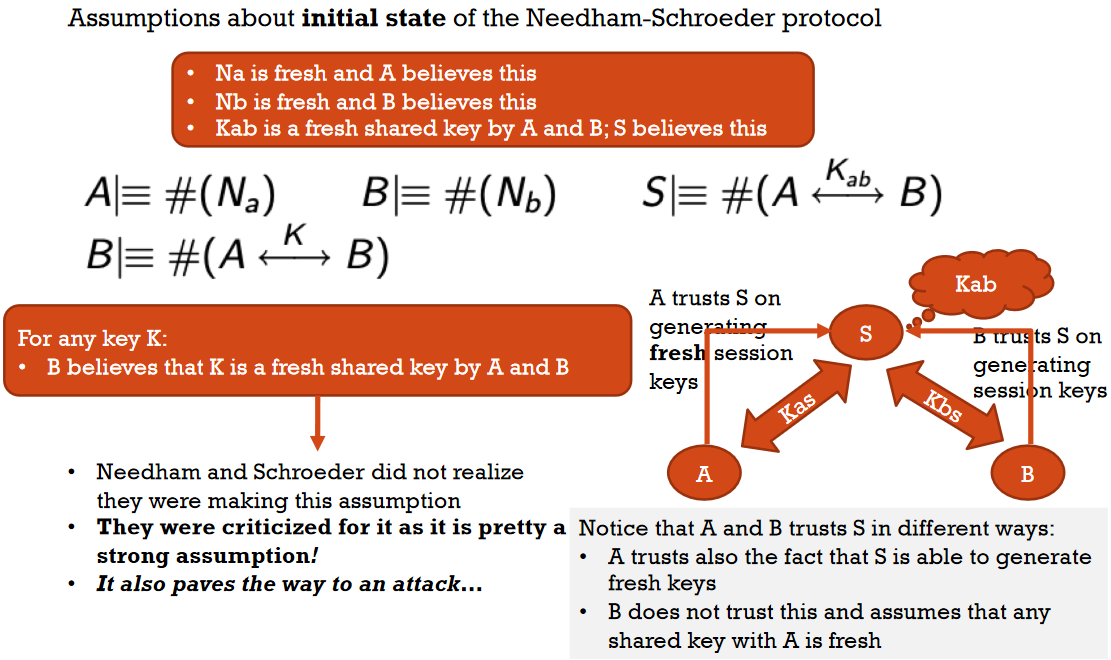
\includegraphics[width=0.7\linewidth]{Images/Chapter4/formalization23}
	\caption{Formalization 2.3}
	\label{fig:formalization23}
\end{figure}

Needham and Schroeder did not realize they were making this assumption.

\section{Deduction}

\begin{figure}
	\centering
	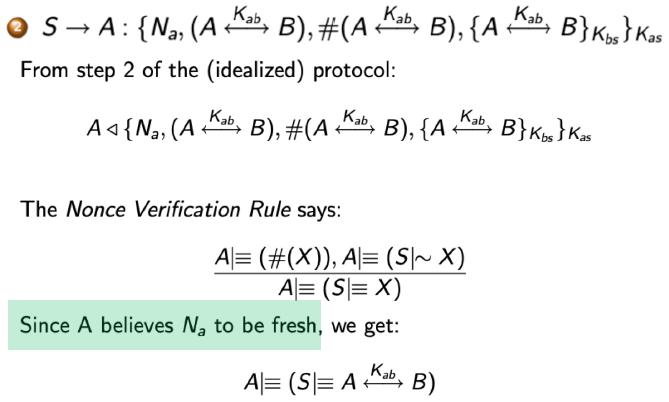
\includegraphics[width=0.7\linewidth]{Images/Chapter4/deduction1}
	\caption{Deduction 1}
	\label{fig:deduction1}
\end{figure}
\begin{figure}
	\centering
	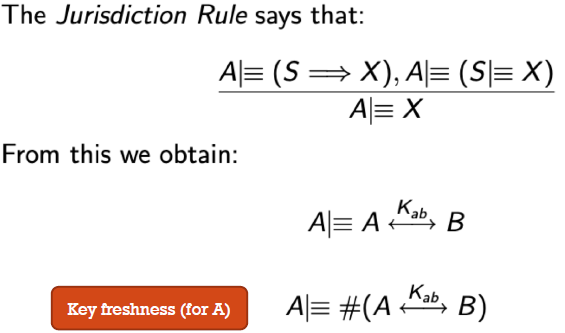
\includegraphics[width=0.7\linewidth]{Images/Chapter4/deduction2}
	\caption{Deduction 2}
	\label{fig:deduction2}
\end{figure}

\begin{figure}
	\centering
	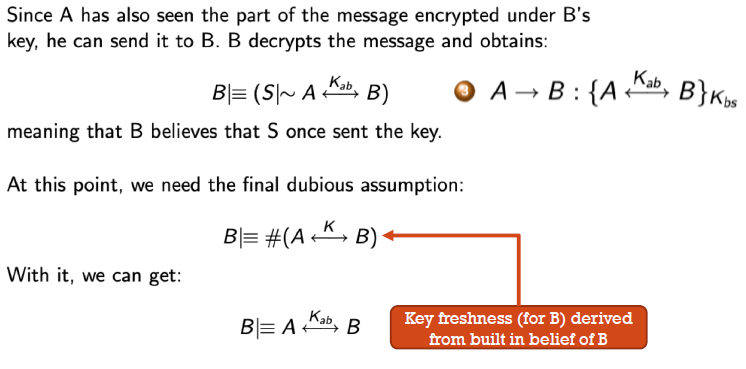
\includegraphics[width=0.7\linewidth]{Images/Chapter4/deduction3}
	\caption{Deduction 3}
	\label{fig:deduction3}
\end{figure}

\begin{figure}
	\centering
	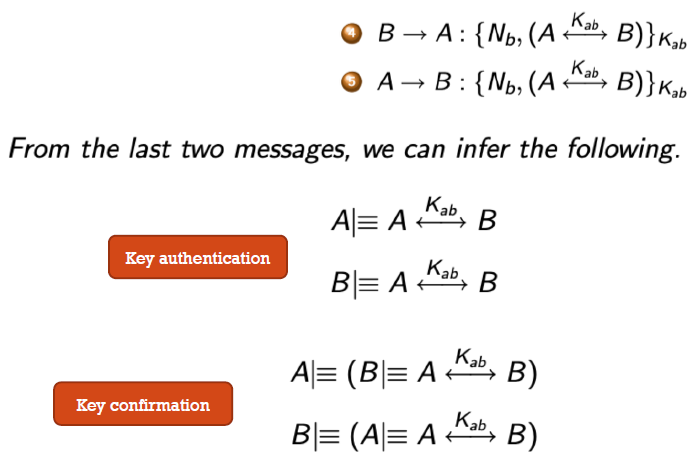
\includegraphics[width=0.7\linewidth]{Images/Chapter4/deduction4}
	\caption{Deduction 4}
	\label{fig:deduction4}
\end{figure}

The assumption $ B \mid \equiv \#(A \Leftrightarrow^K B)$ is dubious because it is different from all other freshness assumptions since those were all based on values that the believing principal had herself generated. This one expresses $B$ belief that a random value someone else has generated is fresh! The consequence of this strange assumption is the attack described above where an attacker is assumed to be able to compromise an old session key. Since $B$ is ready to accept the freshness of any key generated by $S$, it is willing to accept also the compromised key that can be replayed by the attacker that was able to compromise it.



The attack relies on the fact that $B$ has no way to actually be assured that message 3 is fresh. An attacker could spend whatever time is needed to break the session key $K_{AB}$ as long as it can do so within the lifetime of $K_{BS}$, it can run the replay attack described above. $B$ will think it has confirmed sharing $K_{AB}$ with $A$, when in reality $A$ is not present and the attacker knows the key. Notice that the replay attack is not directly uncovered by a BAN analysis of the protocol; rather the analysis shows that the protocol cannot achieve any sort of authentication for B without making the dubious assumption that underlies the attack.

BAN logic is a belief system and it is much different from a knowledge system. Knowledge systems have an inference rule of the form "if a principal known p, then p is true". Belief systems do not have this rule, since a belief in p says nothing about the truth or falsity of p.

In BAN logic, it is assumed that all principals taking part in a protocol are honest, in the sense that each principal believes in the truth of each message it sends. Unfortunately, this assumption is far from being reasonable in presence of attackers.

%TODO: Add details on the analysis of the Needham-Schroeder protocol 56..73 6-KeyDistribution-2p.pdf